\documentclass[utf8]{article}

\usepackage{preamble}

\graphicspath{{figures/}}
\makeatletter
\def\input@path{{figures/}{tables/}}
\makeatother

\def\bfig#1#2{\expandafter\gdef\csname fig-#1\endcsname{\begin{figure}[ht]#2\label{#1}\end{figure}}}
\def\fref#1{\csname fig-#1\endcsname\Cref{#1}}

\bfig{fig:n3t553_start_sites}{
    \centering
    \begin{subfigure}{3cm}
        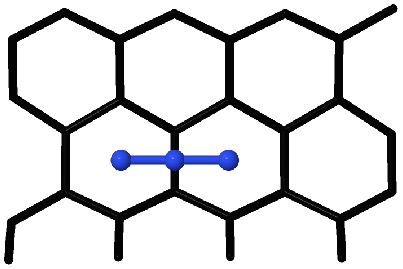
\includegraphics[width=\textwidth]{n3_t553_start_b-cropped.pdf}
        \caption{bond}
    \end{subfigure}
    \hspace{1cm}
    \begin{subfigure}{3cm}
        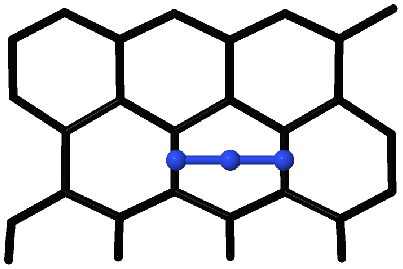
\includegraphics[width=\textwidth]{n3_t553_start_h-cropped.pdf}
        \caption{hollow}
    \end{subfigure}
    \hspace{1cm}
    \begin{subfigure}{3cm}
        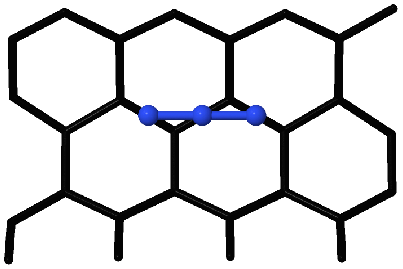
\includegraphics[width=\textwidth]{n3_t553_start_z-cropped.pdf}
        \caption{zigzag}
    \end{subfigure}
    \caption{Starting sites of the bond, hollow and zigzag geometries, respectively.}
}

\bfig{fig:n3t553_start_center}{
    \centering
    \begin{subfigure}{3cm}
        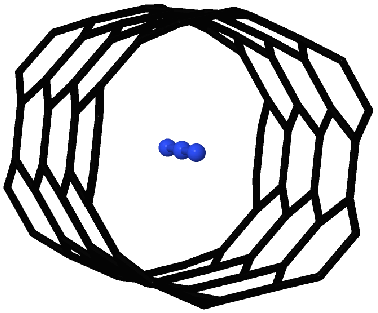
\includegraphics[width=\textwidth]{n3_t553_start_c-cropped.pdf}
    \end{subfigure}
    \hspace{1cm}
    \begin{subfigure}{3cm}
        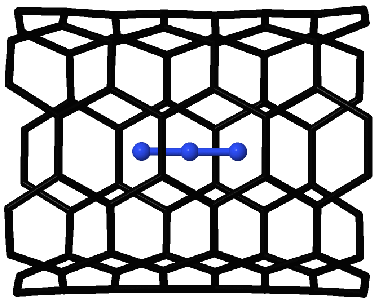
\includegraphics[width=\textwidth]{n3_t553_start_c_side-cropped.pdf}
    \end{subfigure}
    \caption{Central starting geometry (c). Note that the nanotube model has dangling hydrogen atoms at the two ends which are not shown here.}
}

\bfig{fig:n3t553_geom_parms}{
    \centering
    \begin{subfigure}{4.7cm}
        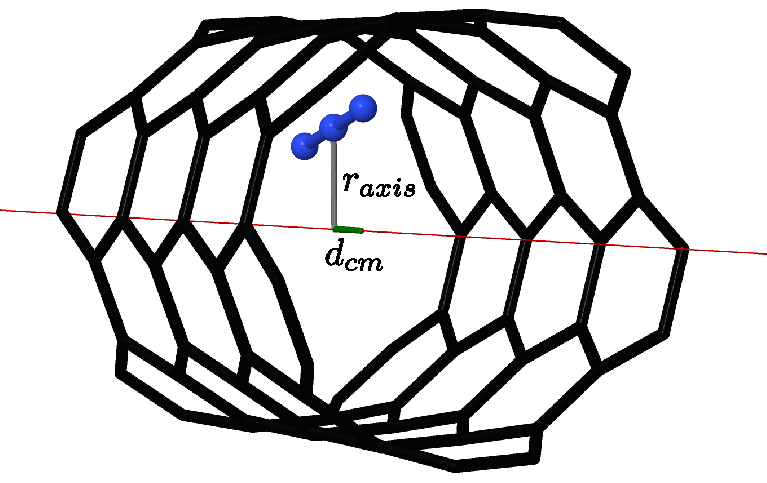
\includegraphics[width=\textwidth]{n3_t553_dist-cropped.pdf}
    \end{subfigure}
    \hspace{1cm}
    \begin{subfigure}{4cm}
        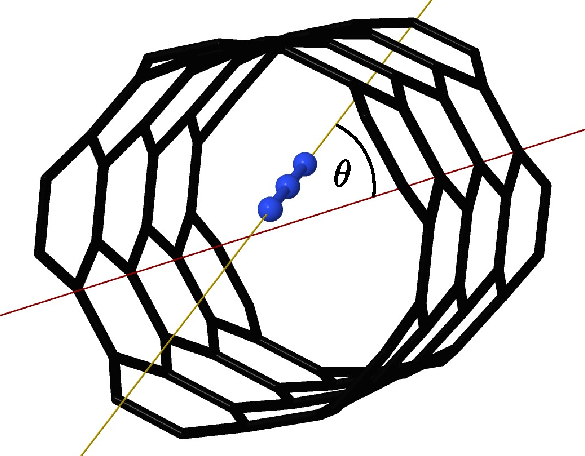
\includegraphics[width=\textwidth]{n3_t553_angle-cropped.pdf}
    \end{subfigure}
    \caption{Geometrical parameters.}
}

\def\btab#1#2{\expandafter\gdef\csname tab-#1\endcsname{\begin{table}[ht]#2\label{#1}\end{table}}}
\def\tref#1{\csname tab-#1\endcsname\Cref{#1}}

\btab{tab:geom_comp}{
    \centering
    \begin{tabular}{crrrrr}
        \toprule
        \textit{$\Lambda$} & site & $d_{cm}$ (\AA) & $r_{axis}$ (\AA) & $\theta$ ($^{\circ}$) & $\Delta E_{int}$ (kcal/mol) \\
        \midrule
        \multirow{3}{*}{3} & \textit{bond} & $ 0.018$ & $ 0.002$ & $0.06$ & $-0.001$ \\
        ~ & \textit{hollow}                & $ 0.002$ & $ 0.003$ & $0.04$ & $ 0.000$ \\
        ~ & \textit{zigzag}                & $ 0.000$ & $ 0.003$ & $0.27$ & $-0.002$ \\
        \midrule
        \multirow{3}{*}{5} & \textit{bond} & $ 0.604$ & $ 0.009$ & $0.32$ & $ 0.112$ \\
        ~ & \textit{hollow}                & $-0.144$ & $ 0.002$ & $0.32$ & $ 0.017$ \\
        ~ & \textit{zigzag}                & $ 0.000$ & $ 0.003$ & $0.43$ & $ 0.000$ \\
        \midrule
        \multirow{3}{*}{7} & \textit{bond} & $ 0.470$ & $ 0.029$ & $1.10$ & $ 0.588$ \\
        ~ & \textit{hollow}                & $-0.233$ & $ 0.027$ & $0.54$ & $ 0.417$ \\
        ~ & \textit{zigzag}                & $ 0.001$ & $ 0.038$ & $0.18$ & $ 0.363$ \\
        \midrule
        \multirow{3}{*}{9} & \textit{bond} & $ 0.622$ & $ 0.015$ & $0.74$ & $ 0.400$ \\
        ~ & \textit{hollow}                & $-1.304$ & $ 0.003$ & $0.17$ & $ 0.030$ \\
        ~ & \textit{zigzag}                & $-0.007$ & $ 0.004$ & $0.53$ & $ 0.141$ \\
        \bottomrule
    \end{tabular}
    \caption{Geometrical parameters and interaction energy difference with respect to the (c) geometry. Note that the $d_{cm}$, $r_{axis}$ and $\theta$ are all zero for the (c) geometry.}
}

\btab{tab:eint_cnt55x_cc-pvtz}{
    \centering
    \begin{tabular}{r cccccc}
        \toprule
        $\Lambda$-CNT & 3-CNT     & 5-CNT     & 7-CNT     & 9-CNT    & 11-CNT   & 13-CNT   \\
        occ./virt.    & 260/2800  & 380/4000  & 500/5200  & 620/6400 & 740/7600 & 860/8800 \\
        \midrule
        RI-B97D3      & $-30.80$  & $-38.29$  & $-42.58$  & $-45.73$ & $-48.06$ & $-49.94$ \\
        \textit{Time} & 27m       & 50m       & 1h20m     & 2h20m    & 4h12m    & 7h35m    \\
        \vspace{1mm} \\
        RI-SCS-MP2    & $-34.56$  & $-43.36$  & $-$       & $-$      & $-$      & $-$ \\
        \textit{Time} & 8h        & 36h (8cpus) & $-$     & $-$      & $-$      & $-$ \\
        \bottomrule
    \end{tabular}
    \caption{CP-corrected unrelaxed interaction energies of N$_3^-$ confined inside a $(5,5)$ SWCNT of increasing length. The azide anion is placed perfectly in the center of the nanotube, parallel to the principal axis. The basis set use is the \textbf{cc-pvtz} with the addition of diffuse functions (aug-) on the anion. All energies are given in kcal/mol.}
}

\btab{tab:eint_cnt55x_cc-pvdtz}{
    \centering
    \begin{tabular}{r cccccc}
        \toprule
        $\Lambda$-CNT & 3-CNT     & 5-CNT     & 7-CNT     & 9-CNT    & 11-CNT   & 13-CNT   \\
        occ./virt.    & 260/1400  & 380/1900  & 500/2500  & 620/3000 & 740/3600 & 860/4150 \\
        \midrule
        RI-B97D3      & $-26.26$  & $-33.97$  & $-38.50$  & $-41.85$ & $-44.36$ & $-46.36$ \\
        \textit{Time} & 9m        & 20m       & 33m       & 45m      & 62m      & 1h25m    \\
        \vspace{1mm} \\
        RI-SCS-MP2    & $-29.77$  & $-38.87$  & $-43.58$  & $-47.07$ & $-49.88$ & $-$ \\
        \textit{Time} & 1h40m     & 6h        & 10h       & 24h      & 50h20m   & $-$ \\
        \vspace{1mm} \\
        DLPNO-CCSD(T) & $-31.96$  & $-$       & $-$       & $-$      & $-$      & $-$ \\
        \textit{Time} & 28h       & $-$       & $-$       & $-$      & $-$      & $-$ \\
        \bottomrule
    \end{tabular}
    \caption{CP-corrected unrelaxed interaction energies of N$_3^-$ confined inside a $(5,5)$ SWCNT of increasing length. The azide anion is placed perfectly in the center of the nanotube, parallel to the principal axis. The basis set use is the \textbf{cc-pvdz} on the nanotube and the aug-cc-pvtz on the anion. All energies are given in kcal/mol.}
}

\btab{tab:ILJ_parms}{
    \centering
    \begin{tabular}{l cccc}
        \toprule
        atom types      & $\epsilon$  & $r_0$     & $\beta$ & $m$ \\
        \midrule
        C--N$_{1,3}$     & 5.205       & 3.994     & 6--9    & 6.0 \\
        C--N$_{2}$       & 3.536       & 3.828     & 6--9    & 6.0 \\
        \bottomrule
    \end{tabular}
    \caption{ILJ parameters for the interaction of N$_{3}^{-}$ confined inside a carbon nanotube. Different values of $\beta$ are tested.}
}

\btab{tab:n3_t553_ILJ_eint}{
    \centering
    \begin{tabular}{l rrr}
        \toprule
        Terms                & $\beta = 7.0$ & $\beta = 8.0$ & $\beta = 9.0$ \\
        \midrule
        $V_{ILJ}$ [kcal/mol] & $-10.90$      & $-9.68$       & $-8.37$      \\
        $V_{els}$ [kcal/mol] & $+42.24$      & $+42.24$      & $+42.24$      \\
        $V_{ind}$ [kcal/mol] & $-52.91$      & $-52.91$      & $-52.91$      \\
        \midrule
        $V_{tot}$ [kcal/mol] & $-21.57$      & $-20.35$      & $-19.04$      \\
        \midrule
        $V_{SCS-MP2/DZP}$ [kcal/mol]       & \multicolumn{3}{c}{$-26.94$}  \\
        $V_{SCS-MP2/TZP}$ [kcal/mol]       & \multicolumn{3}{c}{$-34.52$}  \\
        $V_{L-CCSD(T)/DZP}$ [kcal/mol]       & \multicolumn{3}{c}{$-28.84$} \\
        $\bar{V}_{L-CCSD(T)/TZP}$ [kcal/mol] & \multicolumn{3}{c}{$-36.42$} \\
        \bottomrule
    \end{tabular}
    \caption{Interaction energies for N$_3^-$ confined inside a 3-CNT(5,5).}
}

\btab{tab:n3_t555_ILJ_eint}{
    \centering
    \begin{tabular}{l rrr}
        \toprule
        Terms                & $\beta = 7.0$ & $\beta = 8.0$ & $\beta = 9.0$ \\
        \midrule
        $V_{ILJ}$ [kcal/mol] & $-12.33$      & $-11.15$      & $-9.89$       \\
        $V_{els}$ [kcal/mol] & $+27.55$      & $+27.55$      & $+27.55$      \\
        $V_{ind}$ [kcal/mol] & $-56.83$      & $-56.83$      & $-56.83$      \\
        \midrule
        $V_{tot}$ [kcal/mol] & $-41.61$      & $-40.43$      & $-39.16$      \\
        \midrule
        $V_{SCS-MP2/DZP}$ [kcal/mol]       & \multicolumn{3}{c}{$-36.06$}  \\
        $V_{SCS-MP2/TZP}$ [kcal/mol]       & \multicolumn{3}{c}{$-43.36$}  \\
        $V_{L-CCSD(T)/DZP}$ [kcal/mol]       & \multicolumn{3}{c}{$-37.08$} \\
        $\bar{V}_{L-CCSD(T)/TZP}$ [kcal/mol] & \multicolumn{3}{c}{$-44.34$} \\
        \bottomrule
    \end{tabular}
    \caption{Interaction energies for N$_3^-$ confined inside a 5-CNT(5,5).}
}

\btab{tab:n3_t557_ILJ_eint}{
    \centering
    \begin{tabular}{l rrr}
        \toprule
        Terms                & $\beta = 7.0$ & $\beta = 8.0$ & $\beta = 9.0$ \\
        \midrule
        $V_{ILJ}$ [kcal/mol] & $-12.79$      & $-11.66$      & $-10.46$      \\
        $V_{els}$ [kcal/mol] & $+18.70$      & $+18.70$      & $+18.70$      \\
        $V_{ind}$ [kcal/mol] & $-57.71$      & $-57.71$      & $-57.71$      \\
        \midrule
        $V_{tot}$ [kcal/mol] & $-51.81$      & $-50.68$      & $-49.48$      \\
        \midrule
        $V_{SCS-MP2/DZP}$ [kcal/mol]       & \multicolumn{3}{c}{$-40.81$}  \\
        $V_{SCS-MP2/TZP}$ [kcal/mol]       & \multicolumn{3}{c}{$-47.84$}  \\
        $V_{L-CCSD(T)/DZP}$ [kcal/mol]       & \multicolumn{3}{c}{$-41.91$}  \\
        $\bar{V}_{L-CCSD(T)/TZP}$ [kcal/mol] & \multicolumn{3}{c}{$-48.94$}  \\
        \bottomrule
    \end{tabular}
    \caption{Interaction energies for N$_3^-$ confined inside a 7-CNT(5,5).}
}

\btab{tab:n3_t559_ILJ_eint}{
    \centering
    \begin{tabular}{l rrr}
        \toprule
        Terms                & $\beta = 7.0$ & $\beta = 8.0$ & $\beta = 9.0$ \\
        \midrule
        $V_{ILJ}$ [kcal/mol] & $-12.73$      & $-11.58$      & $-10.37$      \\
        $V_{els}$ [kcal/mol] & $+13.64$      & $+13.64$      & $+13.64$      \\
        $V_{ind}$ [kcal/mol] & $-58.27$      & $-58.27$      & $-58.27$      \\
        \midrule
        $V_{tot}$ [kcal/mol] & $-57.36$      & $-56.22$      & $-55.00$      \\
        \midrule
        $V_{SCS-MP2/DZP}$ [kcal/mol] & \multicolumn{3}{c}{$-44.31$}  \\
        \bottomrule
    \end{tabular}
    \caption{Interaction energies for N$_3^-$ confined inside a 9-CNT(5,5).}
}

\btab{tab:n3_t5511_ILJ_eint}{
    \centering
    \begin{tabular}{l rrr}
        \toprule
        Terms                & $\beta = 7.0$ & $\beta = 8.0$ & $\beta = 9.0$ \\
        \midrule
        $V_{ILJ}$ [kcal/mol] & $-12.67$      & $-11.52$      & $-10.28$      \\
        $V_{els}$ [kcal/mol] & $+10.60$      & $+10.60$      & $+10.60$      \\
        $V_{ind}$ [kcal/mol] & $-58.54$      & $-58.54$      & $-58.54$      \\
        \midrule
        $V_{tot}$ [kcal/mol] & $-60.61$      & $-59.46$      & $-58.23$      \\
        \midrule
        $V_{SCS-MP2/DZP}$ [kcal/mol] & \multicolumn{3}{c}{$-47.12$}  \\
        \bottomrule
    \end{tabular}
    \caption{Interaction energies for N$_3^-$ confined inside a 11-CNT(5,5).}
}

\btab{tab:n3_t5513_ILJ_eint}{
    \centering
    \begin{tabular}{l rrr}
        \toprule
        Terms                & $\beta = 7.0$ & $\beta = 8.0$ & $\beta = 9.0$ \\
        \midrule
        $V_{ILJ}$ [kcal/mol] & $-$      & $-$      & $-$      \\
        $V_{els}$ [kcal/mol] & $-$      & $-$      & $-$      \\
        $V_{ind}$ [kcal/mol] & $-$      & $-$      & $-$      \\
        \midrule
        $V_{tot}$ [kcal/mol] & $-$      & $-$      & $-$      \\
        \midrule
        $V_{SCS-MP2/DZP}$ [kcal/mol] & \multicolumn{3}{c}{$-49.16$}  \\
        \bottomrule
    \end{tabular}
    \caption{Interaction energies for N$_3^-$ confined inside a 11-CNT(5,5).}
}

\btab{tab:n3_t553_dft_comp}{
    \centering
    \scriptsize
    \begin{tabular}{cccccccc}
        \toprule
        SCS-MP2 & B97-D3  & BLYP-D3 & rPW86PBE-D3 & wB97X-D3 & TPSS0-D3 & B3LYP-D3 & PW6B95-D3  \\
        \midrule
        $-2.19$ & $-5.70$ & $-4.99$ & $-6.89$     & $-6.28$  & $-8.08$  & $-6.88$  & \\
        \bottomrule
    \end{tabular}
    \caption{Interaction energy differences in kcal/mol of various density functionals with respect to the reference DLPNO-CCSD(T) value for N$_3^-$ confined inside a 3-CNT(5,5).}
}

\btab{tab:els_basis_comp}{
    \centering
    \begin{tabular}{c ccc}
        \toprule
        $\Lambda$ & cc-pvdz & cc-pvtz & cc-pvqz \\
        \midrule
        3         & $48.20$ & $42.24$ & $45.20$ \\
        5         & $31.46$ & $27.55$ & $28.78$ \\
        \bottomrule
    \end{tabular}
    \caption{Comparison of electrostatic contribution in kcal/mol with respect to the basis set used in the calculation to obtain the partial atomic charges.}
}


%
% A second series of test has been done by resetting the term $\tfrac{n_2}{n_2 - 4}$, which depends on $\beta$ and therefore will change accordingly.
% \Cref{tab:eint_geo_1_ind_beta} shows the results in this case.
% %
% \begin{table}
%     \centering
%     \begin{tabular}{l|rrrr}
%         $E_{int}$            & $\beta = 6.0$ & $\beta = 7.0$ & $\beta = 8.0$ & $\beta = 9.0$ \\
%         \midrule
%         $V_{ILJ}$ [meV]      &  -569.17      &  -517.63      &  -462.66      &  -403.66      \\
%         $V_{ILJ}$ [kcal/mol] &   -13.12      &   -11.94      &   -10.67      &    -9.31      \\
%         $V_{ind}$ [meV]      & -4033.24      & -3818.14      & -3657.00      & -3531.54      \\
%         $V_{ind}$ [kcal/mol] &   -93.01      &   -88.05      &   -84.33      &   -81.44      \\
%         \midrule
%         $E_{int}$ [meV]      & -4602.40      & -4335.77      & -4119.67      & -3935.20      \\
%         $E_{int}$ [kcal/mol] &  -106.13      &   -99.98      &   -95.00      &   -90.75
%     \end{tabular}
%     \caption{Interaction energies computed using ILJ and the induction term for different $\beta$ values. The term $\tfrac{n_2}{n_2 - 4}$ in the induction potential was let free to vary. The reference MP2 value is -32.31 kcal/mol (-1401.13 meV).}
%     \label{tab:eint_geo_1_ind_beta}
% \end{table}
% %
% A third series of calculations has been performed using NBO charges calculated on the MP2 density; namely $q_1 = q_3 = -0.51$ and $q_2 = -0.01$. Note that the total charge on the trinitrogen anion is not exactly $-1$, but a tiny donation from the nanotube to the confined molecule has occurred. The results for this charge distributions are not listed because for both cases considered above, the resulting interaction energies are constantly lower (i.e. more favorable) by about 4 to 6 kcal/mol.


\title{\LARGE Static and Dynamics of the Azide Anion Confined in an Armchair Carbon Nanotube}

\author{Stefano Battaglia}

\begin{document}

\maketitle

\section{Introduction}
Introduction

\section{Computational Details}
The computational details section is divided in two parts.
The first one describes the details of the \textit{ab-initio} calculations performed in order to obtain accurate interaction energies and partial atomic charges of the two fragments.
The second one describes the analytical potential employed in the molecular dynamics (MD) simulations and assesses its performance against the \textit{ab-initio} values.


\subsection{\textit{Ab-Initio}}
At \textit{ab-initio} level, carbon nanotubes (CNTs) have been treated as finite-size systems and the two open ends have been capped with hydrogen atoms in order to fill out the valence shell. Only one type of armchair nanotube has been considered, with chiral indices $(5,5)$. In order to obtain converged values with respect to the length of the nanotube, CNTs with different number of units have been studied. We introduce here the notation $\Lambda$-$(5,5)$CNT to label a nanotube composed by $\Lambda$ units, where a single unit corresponds to a [$10$]cyclophenacene (see FIGURE).


\subsubsection{Geometries}
The geometries of the nanotubes and the azide anion have been optimized using restricted Kohn-Sham density functional theory (DFT), employing the B97D3 exchange-correlation functional with Becke-Johnson damping\cite{Grimme2010,Grimme2011}.
For both fragments Dunning's triple-$\zeta$ cc-pVTZ basis set\cite{DunningJr1989} has been used, with the addition of diffuse functions (aug-)\cite{Kendall1992} in the case of the \ntm fragment.\\
The nanotubes geometries retained the high $D_{5d}$ symmetry, with both parallel and perpendicular (to the principal axis) C--C bonds showing the typical alternation pattern of these systems when treated with open boundary conditions\cite{Zhou2004,Galano2006}. As the length of the nanotube increases, the average C--C bond length approaches the experimental value of 1.421 \AA\ [REFERENCE].\\
The relaxed \ntm geometry has linear $D_{\infty h}$ symmetry, with an N--N bond length of $1.1874$ \AA, which is in excellent agreement with the experimental gas phase value of $1.1884$ \AA\cite{Polak1987}.\\
All the optimizations just mentioned have been performed using the Gaussian 09 software package, revision d01\cite{g09}, using the default convergence thresholds, the ultrafine grid for the integral quadrature and spherical \textit{d} and \textit{f} basis functions.


\subsubsection{Interaction Energies}
In order to construct the classical force field (cf. Molecular Dynamics section), the most important parameter to obtain is the interaction energy of the the guest \ntm ion and the host carbon nanotube at the optimal adsorption distance.
In this contribution, all interaction energies computed using first principles methods have been evaluated according to the formula
%
\begin{equation}
    E_{int} = E_{complex} - (E_{cnt} + E_{azide}) \label{eq:eint}
\end{equation}
%
where the fragment energies $E_{cnt}$ and $E_{azide}$ have been computed in the basis set of the complex system, thus correcting the basis set superposition error according to the Boys and Bernardi scheme\cite{Boys1970}.
Relaxation effects on the two interacting fragments have not been taken into account, although it has been recently shown that they contribute only in the order of 1--2 kcal/mol\cite{Battaglia2017a} to $E_{int}$ and thus do not substantially modify the overall picture.\\
To locate the minimum of the potential energy surface (PES), a series of constrained optimizations involving nanotubes of lengths between 3 and 9 units has been performed. In these optimizations, the optimal geometry of the two fragments has been kept frozen and only their relative distance and orientation have been optimized, thus locating the adsorption distance.
This series of optimizations has been performed using the ORCA 4 program package\cite{ORCA} at the same level of theory as before, besides employing the smaller cc-pVDZ basis set on the nanotube, the resolution of the identity technique for the Coulomb matrix using the auxiliary basis def2/J by Weigend \textit{et al.}\cite{Weigend2006}.\\
Remarkably, it turns out that in the particular case of an azide anion confined inside a $(5,5)$CNT, the geometry with the \ntm molecule placed exactly in the center of the nanotube, aligned to its principal axis, results to be a local minimum. Moreover, the difference between this minimum and the lowest minimum found is at most less than $0.6$ kcal/mol for the nanotubes studied. For this reason, the geometry with the \ntm molecule placed in the center of the CNTs has been used for the calculation of $E_{int}$ at higher levels of theory and for nanotubes longer than 9 units.
For a detailed explanation of the structure optimizations, the criteria used to compare them and all the geometries, we point the reader to the Supplementary Information.\\

%%%%
As we are dealing with finite size CNTs, it is important to study the dependence of the interaction energy with respect to the length of the nanotube. In particular, given that the confined species is negatively charged, one expects a slower convergence compared to neutral systems due to the typically more diffuse electron density of anions.\\
Accurate interaction energies have been calculated at wave function level of theory, using the density-fitted spin-component-scaled MP2 method (RI-SCS-MP2)[REFERENCE] and the local coupled cluster method DLPNO-CCSD(T) as implemented in the ORCA 4 program package\cite{Riplinger2013,Riplinger2016}. Calculations have been performed using the cc-pVDZ or the cc-pVTZ basis set (where computationally feasible) and in both cases diffuse functions (aug-) have been added on the \ntm species.\\
\fref{fig:n3t55x_ab-initio_eint} depicts the results obtained for nanotubes of different lengths, where it is immediately clear that interaction energy shows a slow convergence rate with respect to $\Lambda$.
In order to obtain accurate interaction energies within a sufficiently large basis set, extrapolated DLPNO-CCSD(T)/cc-pVTZ values have been obtained using the following formula
%
\begin{equation}
    E_{CC}(pVTZ) \approx E_{MP2}(pVTZ) + (E_{CC}(pVDZ) - E_{MP2}(pVDZ)) \label{eq:basis_extr}
\end{equation}
%
where it is assumed that the correlation energy difference between the two methods is constant with respect to the basis set used.
This approach has allowed us to obtain approximate accurate values for nanotubes of length 3, 5 and 7. Nonetheless, as it can be seen from the RI-SCS-MP2/cc-pVDZ curve in \Cref{fig:n3t55x_ab-initio_eint}, $E_{int}$ still significantly decreases with the addition of extra nanotube units.
Therefore, in order to be able to extrapolate the DLPNO-CCSD(T)/cc-pVTZ confinement energy inside an arbitrary $\Lambda$-(5,5) nanotube we use the following formula
%
\begin{equation}
    E_{int}(\Lambda) = \frac{a\Lambda}{b + \Lambda} \label{eq:length_extr}
\end{equation} 
%
where $a$ and $b$ are two fitting parameters to be determined.
\Cref{eq:length_extr} is the simplest formula which satisfies the condition $E_{int}(0) = 0$ and provides an estimate for the infinitely long nanotube through the parameter $a$.\\
The solid lines in \Cref{fig:n3t55x_ab-initio_eint} show the non-linear least square fits to the RI-SCS-MP2/cc-pVDZ and the approximated DLPNO-CCSD(T)/cc-pVTZ interaction energies computed according to \cref{eq:basis_extr}.
The extrapolated value for $E_{int}$ in the limit of an infinitely long CNT is $-65.93$ kcal/mol.
For a detailed explanation of the parameters used in the calculation and the tests performed to assess the validity of our approach, we point the reader to the Supplementary Information.\\


\subsection{Molecular Dynamics}
The Improved Lennard-Jones (ILJ) potential\cite{Pirani2008} is given by
%
\begin{equation}
    V_{ILJ}(r_{ij}) = \epsilon \left[ \frac{m}{n(r_{ij})-m} \cdot \Big( \frac{r_0}{r_{ij}} \Big)^{n(r_{ij})} -
                                 \frac{n(r_{ij})}{n(r_{ij})-m} \cdot \Big( \frac{r_0}{r_{ij}} \Big)^{m} \right]
\end{equation}
%
where
%
\begin{equation}
    n(r_{ij}) = \beta + 4.0 \cdot \Big( \frac{r_{ij}}{r_0} \Big)^2
\end{equation}
%
and $r_{ij}$ is the distance between atom $i$ in the carbon nanotube and atom $j$ in the \ntm molecule. The parameters $r_0$ and $\epsilon$ are set according to the atoms interacting, $\beta$ is a free parameter used to fit the potential to experimental or numerical values, while $m$ is set according the to the partial charges of the interacting species.
Since the azide anion has a total negative charge of $-1$, one has to introduce a non-bonded term in the potential which accounts for the induced polarization on the carbon nanotube due to the excess negative charge of the anion.
The potential term $V_{ind}$ describing the dipole induced by the $\text{N}_3^-$ anion on a neutral fragment is given by
%
\begin{equation}
    V_{ind}(r_{i1},r_{i2},r_{i3}) = - \frac{1}{2} \cdot \alpha \cdot f(r_{i1},r_{i2},r_{i3})
                        \left[ \frac{q_1}{r_{i1}^2} + \frac{q_2}{r_{i2}^2} + \frac{q_3}{r_{i3}^2} \right]^2
\end{equation}
%
where $r_{i1}$, $r_{i2}$ and $r_{i3}$ are the distances between atom $i$ of the neutral species and the three nitrogen atoms of the azide anion, $q_1$, $q_2$ and $q_3$ are the partial charges on the nitrogen atoms, $\alpha$ is the polarizability per volume of the atoms in the neutral species and $f(r_{i1},r_{i2},r_{i3})$ is a damping factor.\\  % $f(R_{i,2}) = \frac{n(R_{i,2})}{n(R_{i,2}) - 4}$
By saturating the CNT with hydrogen atoms, the two ends of the nanotube result significantly polarized with partial atomic charges in the range of $\pm 0.2$.
As a consequence, the \ntm interacts through the usual Coulomb potential with the partial atomic charges on the nanotube, giving rise to an additional term $V_{els}$ describing this electrostatic potential as
%
\begin{equation}
    V_{els}(r_{ij}) = \frac{q_i q_j}{r_{ij}}
\end{equation}
%
This \textit{artificial} term clearly vanishes when considering infinitely long nanotubes.\\

The total interaction energy $E_{int}$ is finally obtained by summing over all atoms of both fragments for each potential term, as given in the following
%
\begin{align}
    E_{int} = \sum_{i=1}^{N_C + N_H} V^{(i)}_{ind}(r_{i1},r_{i2},r_{i3}) +
              \sum_{j=1}^{N_N} V_{ILJ}^{(ij)}(r_{ij}) + V_{els}(r_{ij})
\end{align}
%
where $N_C$, $N_N$ and $N_H$ correspond to the total number of carbon, nitrogen and hydrogen atoms, respectively.
The superscript $(ij)$ in the ILJ potential term $V_{ILJ}^{(ij)}$ keeps track of the interacting atom types such that the parameters can be accordingly set to the values given in \tref{tab:ILJ_parms} [WHERE DO THESE VALUES COME FROM?].
The values used for the polarizability per volume (in \AA$^{-3}$) appearing in $V^(i)_{ind}$ are given by $\alpha_H = 0.34$ and $\alpha_C = 1.20$ for hydrogen and carbon, respectively.
The partial atomic charges on the azide anion were set to be $q_1 = q_3 = -0.56$ and $1_2 = 0.12$, while for the carbon nanotube they have been obtained through a natural population analysis\cite{Reed1985a} of the electron density calculated at B97D3/cc-pVTZ level of theory.\\

In \fref{fig:n3t55x_comp_eint} it can be seen the direct comparison of the \emph{ab-initio} and the classical potential ($\beta = 8$ and $f(r_{i1},r_{i2},r_{i3}) = 1$) for nanotubes with $\Lambda = 3,5,7,9,11,13$. 
The various components of the classical potential can also be considered separately, and these are listed in \tref{tab:pot_comp} and plotted in \fref{fig:n3t55x_classical_eint} along with the total one and the \emph{ab-initio} one.

piccola modifica

\clearpage

\bibliographystyle{unsrt}
\bibliography{library}

\clearpage
\section{Supplementary Information}
To ensure that the relaxation process did not remain trapped in a local minimum and without knowing a priori the optimal adsorption distance of the N$_3^-$ molecule, the optimization procedure has been started from four different geometries.
In all cases, the anion has been placed parallel to the principal axis of the nanotube.
Three starting geometries were chosen according to possible ``adsorption'' sites in which the central nitrogen atom of the azide was placed either over C--C bonds (\textit{bond} (b) and \textit{zigzag} (z) geometries) or in the center of an hexagonal ring of the CNT wall (\textit{hollow} (h) geometry). The three starting sites are shown in \fref{fig:n3t553_start_sites}, along with their labels that will be used in the following to refer to them. For all three cases, the azide anion has been placed at a distance of about $2.25$\AA\ from the nanotube wall, well below the optimal adsorption distance.
The fourth starting geometry is shown in \fref{fig:n3t553_start_center} and it simply consists in the N$_3^-$ anion placed exactly in the center of the nanotube. We will refer to this starting geometry as \textit{central} (c) geometry.
In order to study the edge effects on the position of the minimum, CNTs of four different lengths have been considered, namely with 3, 5, 7 and 9 units.
The relaxation has been performed again at DFT level using the B97D3 functional, but this time with the smaller cc-pvdz\cite{DunningJr1989} basis set on the carbon nanotube and the aug-cc-pvtz\cite{DunningJr1989} on the N$_3^-$.
The resolution-of-the-identity (RI) approximation has been used to compute the Coulomb matrix, adopting the universal fitting basis set def2/j\cite{Weigend2006}. The calculations have been performed using the ORCA 4 program package\cite{ORCA}.\\
The relaxed structures starting from the (c) geometry correspond to a (local) minimum, as after one optimization step the convergence is reached, with the \ntm anion insignificantly ($\approx 0.002$\AA) shifted out of the principal axis. For this reason we will consider from now on the (c) geometry as the perfectly aligned anion to the principal axis and sitting in the center of the nanotube.
For the three other starting conformations, namely the the (b), (h) and (z) geometries, the relaxation leads to different (local) minima.
In order to analyze the differences in the final structures, three geometrical parameters and an energetic one have been considered.
The geometrical parameters are depicted in \fref{fig:n3t553_geom_parms} and consist in the axial distance $d_{cm}$ between the center of mass of the azide anion and the center of mass of the carbon nanotube, the radial distance $r_{axis}$ of the azide anion center of mass from the principal axis of the nanotube and the angle $\theta$ formed between the principal axis and an imaginary line passing through the external nitrogen atoms of the azide anion.
The energetic parameter is the interaction energy $E_{int}$ between the two fragments, computed as
%
\begin{equation}
    E_{int} = E_{complex} - (E_{cnt} + E_{azide})
\end{equation}
%
and corrected for the basis set superposition error according to the Boys and Bernardi scheme\cite{Boys1970}.
Note that although geometry optimizations have been carried out on the complex systems, the geometry of the two fragments was kept frozen at the optimal fragment conformation, thus the value obtained from \Cref{eq:eint} is only the interaction energy and not the binding energy of the system (i.e. it does not account for deformation effects).\\
The four parameters computed for all systems are listed in \tref{tab:geom_comp}. Since the (c) geometry consists in the azide ion sitting in the exact center of the nanotube, the three conformational parameters are all zero in this case, thus for geometries (b), (h) and (z), the parameters can be considered as differences from the (c) geometry. Accordingly, instead of tabulating the interaction energy for every geometry, the values listed in the last column of \Cref{tab:geom_comp} correspond to the interaction energy difference between the (c) geometry and the other three, i.e. $\Delta E_{int} = E_{int}(c) - E_{int}(site)$. A negative value for $\Delta E_{int}$ means that the interaction energy is more favorable (i.e. stronger) for the (c) geometry, while a positive value the opposite.\\
For all final geometries, the azide anion is found to be almost perfectly aligned to the principal axis of the nanotube since the angle $\theta$ is always very small (below $1^{\circ}$ except in one case), confirming the results presented in \cite{Battaglia2017a}.
Similarly, $r_{axis}$ is also always particularly small (most of the times below $0.01$ \AA), meaning that the anion has the preference to stay approximately at the same distance from the nanotube wall in all directions.
In particular, independently from the length $\Lambda$, the azide ion is adsorbed at a distance of approximately $3.34$ \AA\ (computed as the distance between the \ntm center of mass and the closest side of the wall). This value is significantly larger than the adsorption distance of $3.17$ \AA\ found for the confinement in a larger 3-CNT(6,6), obtained following the same computational procedure.
There are two possible explanations for the difference in the adsorption distance. Either the different curvature of the two nanotubes is such that the forces attracting the ion are stronger in the case of the (6,6) CNT, or in the case of the (5,5) CNT, there is a competition between the attractive forces exerted by the surrounding wall on the azide ion, which eventually stabilizes it at an (almost) equal radial distance in any direction.
The analysis of the curvature effects on the adsorption distance inside the CNT are beyond the scope of this work, and thus not further investigated here [maybe there are refs for other systems, probably H2 and H2O].
The most fluctuating parameter is $d_{cm}$. Clearly, the periodic atomic pattern of the carbon nanotube makes the potential energy surface (PES) of the complex full of local minima, all of which approximately share the same well depth. Apart from the (z) conformation, for which $d_{cm}$ remains virtually unchanged irrespective of the length, it is hard to rationalize the results for the (b) and (h) cases.
The only exception is found for the 3-CNT(5,5), where the two open ends of the nanotube are so close that the energy barriers to move away from the center are particularly steep.
Nonetheless, although the evident difference between the final geometries, the effect observed on the interaction energy, which is our first and most important parameter that we are interested in, is minimal and, importantly, below chemical accuracy ($\approx 1$ kcal/mol).
As it appears a very hard task to find the \emph{global minimum} for this type of systems and considering the small influence observed on the interaction energy as well as remembering that the accuracy of classical parametrized potentials is well below the differences $\Delta E_{int}$ listed in \Cref{tab:geom_comp} [maybe ref?], the central geometry (c) will be used for all interaction energies computed in this work at a higher level of theory and for nanotubes longer than $\Lambda = 9$.\\


In order to test the performance of the classical potential, we have computed the interaction energy between the azide anion and a short 3-CNT(5,5) nanotube at \textit{ab-intio} level and compared it with the result obtained by the potential, as shown in \tref{tab:n3_t553_ILJ_eint}.\\
Similarly, we have compared the interaction energies for the confinement in a longer 5-CNT(5,5), listed in \tref{tab:n3_t555_ILJ_eint}.
Moreover, \tref{tab:n3_t557_ILJ_eint}, \tref{tab:n3_t559_ILJ_eint}, \tref{tab:n3_t5511_ILJ_eint} and \tref{tab:n3_t5513_ILJ_eint} list the results for longer nanotubes.
A comparison of the interaction energy computed by different dft functionals is listed in \tref{tab:n3_t553_dft_comp}, while a comparison of the electrostatic term with respect to the basis set used in the calculation can be seen in \tref{tab:els_basis_comp}.


\end{document}
